\documentclass{article}
\usepackage[english,russian]{babel}
\usepackage[utf8]{inputenc}
\usepackage{indentfirst}
\usepackage{graphicx}
\usepackage{float}
\usepackage[margin=2cm]{geometry}

\begin{document}
\begin{titlepage}
	\begin{center}
    	ГУАП
    	\vspace{0.25cm}

    	КАФЕДРА №51
	\end{center}

    \begin{flushleft}

    	ОТЧЕТ

    	ЗАЩИЩЕН С ОЦЕНКОЙ

		ПРЕПОДАВАТЕЛЬ 


    	\vspace{0.5cm} 

		$\rule{5cm}{0.15mm}$ \hfill $\rule{2.2cm}{0.15mm}$  \hfill $\rule{3.25cm}{0.15mm}$

		должность, уч. степень, звание \hfill подпись, дата \hfill инициалы, фамилия
    \end{flushleft}
    
 	
    \hspace{2cm}

	\begin{center}
    	ОТЧЕТ ПО ЛАБОРАТОРНОЙ РАБОТЕ №13


    	\vspace{1cm}

    	СЕРВЛЕТЫ


    	\vspace{1cm}

    	по курсу: ОСНОВЫ ПРОГРАММИРОВАНИЯ {\MakeUppercase{\romannumeral 2}}
    \end{center}

    \vspace{3cm}

    \begin{flushleft}
    	РАБОТУ ВЫПОЛНИЛ

    	СТУДЕНТ ГР. № 5511 \hfill $\rule{2.2cm}{0.15mm}$  \hfill $\rule{3.25cm}{0.15mm}$

    	\hspace{7.8cm} подпись, дата \hfill инициалы, фамилия
    \end{flushleft}

	\vspace{5cm}   
	\begin{center}
 		Санкт-Петербург, 2017
	\end{center}
\end{titlepage}

\section{Задание}
Реализовать сервлет для работы с записной книжкой. В записной книжке для каждого человека хранится его имя и список телефонов (их может быть несколько). При старте сервлет загружает записную книжку из текстового файла. сервлет должен позволять:

\begin{enumerate}
	\item Просматривать список записей
	\item Добавить нового пользователя
	\item Добавить новый телефон

\end{enumerate}

На главной странице сервлет находится список записей. Вверху страницы ссылки --- добавить. Каждая из ссылок ведет на отдельную страницу, где с помощью элементов <input type="text" name="username" /> в форме вводятся необходимые данные. Для отправки данных сервлету есть кнопка submit. 

В качестве контейнера сервлетов рекомендуется использовать либо сервер Tomcat, либо сервер Jetty

\section{Дополнительное задание}
На сервере хранится набор аватарок. Добавить возможность при добавлении новой записи с помощью радиокнопки выбрать аватарку. Аватарки должны отображаться в списке.

\section{Реализация}
Программа реализована с использованием контейнера сервлетов Apache Tomcat.
Класс PhoneBook наследуется от класс HttpServlet, у него перегружен метод doGet(), который отвечает за отправку Html страницы клиенту. Он, взависимости от запроса, генерирует соответствующий ответ. Этот сервлет связан с URL в файле web.xml. 
Все файлы необходимые для работы с приложением находятся в папке data. Там же и находятся картинки (для доп. задания) и список контактов в виде текстового файла, он загружается при вызове метода init класса PhoneBook и сохраняется после вызова destroy().

\section{Инструкция}
После запуска сервера при посещении страницы localhost:8080/phonebook/ перед пользователем откроется страница с записной книжкой. Снизу присутствует кнопка Add, которая пересылает на форму добавления нового контакта. 
\section{Тестирование}

\subsection{Главная страница с записной книжкой}
\begin{figure}[H]
	\begin{flushleft}
		\centerline{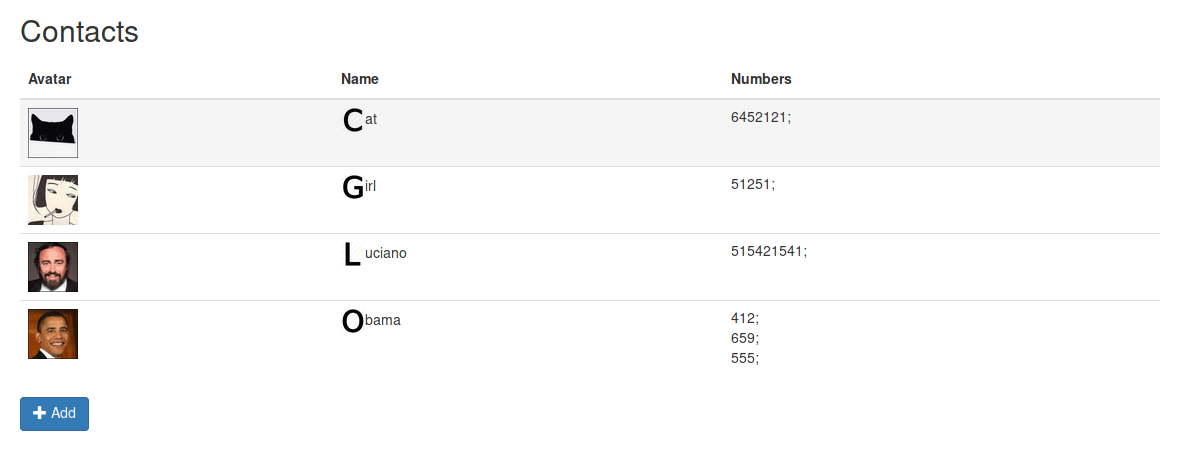
\includegraphics[scale=0.4]{phonebook.png}}
		\caption{Записная книжка}
	\end{flushleft}
\end{figure}
\vspace{3cm}

\subsection{Добавление новой записи}
\begin{figure}[H]
	\begin{flushleft}
		\centerline{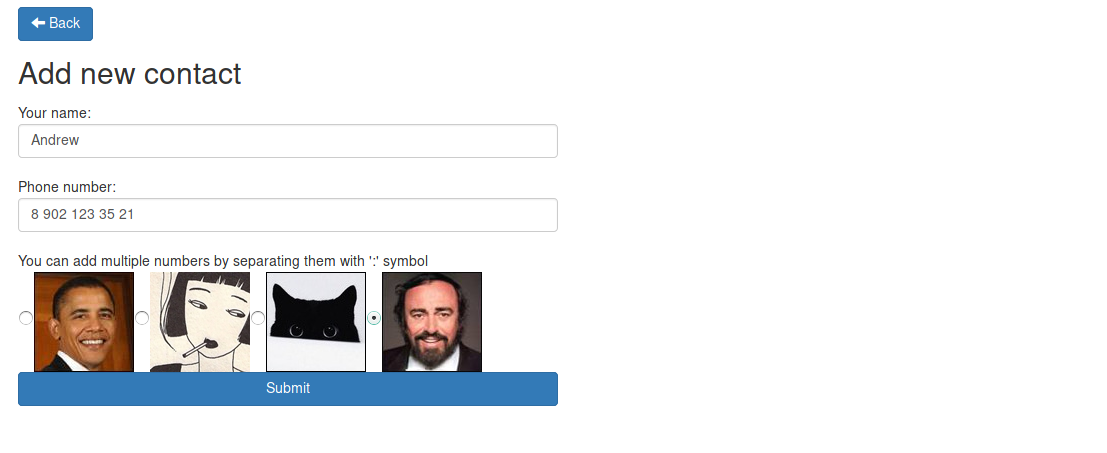
\includegraphics[scale=0.4]{add.png}}
		\caption{Страница добавления новой записи}
	\end{flushleft}
\end{figure}

\subsection{Проверка работоспособности добавления новой записи}
\begin{figure}[H]
	\begin{flushleft}
		\centerline{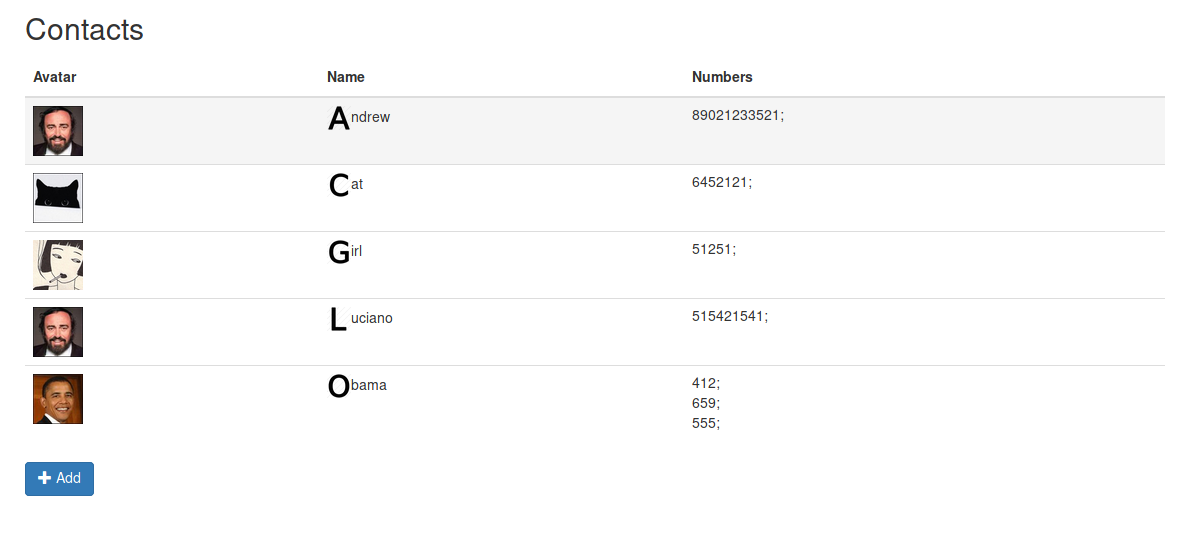
\includegraphics[scale=0.4]{phonebooknew.png}}
		\caption{Записная книжка с только что добавленной записью}
	\end{flushleft}
\end{figure}



\end{document}
